% mnras_template.tex 
%
% LaTeX template for creating an MNRAS paper
%
% v3.0 released 14 May 2015
% (version numbers match those of mnras.cls)
%
% Copyright (C) Royal Astronomical Society 2015
% Authors:
% Keith T. Smith (Royal Astronomical Society)

% Change log
%
% v3.0 May 2015
%    Renamed to match the new package name
%    Version number matches mnras.cls
%    A few minor tweaks to wording
% v1.0 September 2013
%    Beta testing only - never publicly released
%    First version: a simple (ish) template for creating an MNRAS paper

%%%%%%%%%%%%%%%%%%%%%%%%%%%%%%%%%%%%%%%%%%%%%%%%%%
% Basic setup. Most papers should leave these options alone.
\documentclass[fleqn,usenatbib]{mnras}

% MNRAS is set in Times font. If you don't have this installed (most LaTeX
% installations will be fine) or prefer the old Computer Modern fonts, comment
% out the following line
\usepackage{newtxtext,newtxmath}
% Depending on your LaTeX fonts installation, you might get better results with one of these:
%\usepackage{mathptmx}
%\usepackage{txfonts}

% Use vector fonts, so it zooms properly in on-screen viewing software
% Don't change these lines unless you know what you are doing
\usepackage[T1]{fontenc}

% Allow "Thomas van Noord" and "Simon de Laguarde" and alike to be sorted by "N" and "L" etc. in the bibliography.
% Write the name in the bibliography as "\VAN{Noord}{Van}{van} Noord, Thomas"
\DeclareRobustCommand{\VAN}[3]{#2}
\let\VANthebibliography\thebibliography
\def\thebibliography{\DeclareRobustCommand{\VAN}[3]{##3}\VANthebibliography}


%%%%% AUTHORS - PLACE YOUR OWN PACKAGES HERE %%%%%

% Only include extra packages if you really need them. Common packages are:
\usepackage{graphicx}	% Including figure files
\usepackage{amsmath}	% Advanced maths commands
% \usepackage{amssymb}	% Extra maths symbols

%%%%%%%%%%%%%%%%%%%%%%%%%%%%%%%%%%%%%%%%%%%%%%%%%%

%%%%% AUTHORS - PLACE YOUR OWN COMMANDS HERE %%%%%

% Please keep new commands to a minimum, and use \newcommand not \def to avoid
% overwriting existing commands. Example:
%\newcommand{\pcm}{\,cm$^{-2}$}	% per cm-squared

%%%%%%%%%%%%%%%%%%%%%%%%%%%%%%%%%%%%%%%%%%%%%%%%%%

%%%%%%%%%%%%%%%%%%% TITLE PAGE %%%%%%%%%%%%%%%%%%%

% Title of the paper, and the short title which is used in the headers.
% Keep the title short and informative.
\title[S0 type galaxy formation]{S0 type galaxy formation}

% The list of authors, and the short list which is used in the headers.
% If you need two or more lines of authors, add an extra line using \newauthor
\author[Carl Ingebretsen]{
Carl Ingebretsen,$^{1}$\thanks{E-mail: carljingebretsen@arizona.edu}
\\
% List of institutions
$^{1}$University of Arizona\\
}

% These dates will be filled out by the publisher
%\date{Accepted XXX. Received YYY; in original form ZZZ}

% Enter the current year, for the copyright statements etc.
\pubyear{2023}

% Don't change these lines
\begin{document}
\label{firstpage}
\pagerange{\pageref{firstpage}--\pageref{lastpage}}
\maketitle

% Abstract of the paper
\begin{abstract}
In this project, the formation of S0-type galaxies was investigated. In about 3 Gyr the Milky Way and the Andromeda galaxy will merge. This will be the major merger of two similar mass galaxies. It may be possible that the remnant of this merger could be an S0-type galaxy. This possibility was investigated using N-body simulations.
\end{abstract}

% Select between one and six entries from the list of approved keywords.
% Don't make up new ones.
\begin{keywords}
Local Group -- Spiral Galaxy -- Galaxy Merger -- Merger Remnant -- Sersic Profiles
\end{keywords}

%%%%%%%%%%%%%%%%%%%%%%%%%%%%%%%%%%%%%%%%%%%%%%%%%%

%%%%%%%%%%%%%%%%% BODY OF PAPER %%%%%%%%%%%%%%%%%%

\section{Introduction}
Lenticular galaxies (S0-type) are an unusual class of galaxies that seem to incorporate structures of both spiral and elliptical galaxies. A spiral galaxy has a small bulge or bar in the center that is surrounded by arms rich in gas and dust, and with active star formation. An elliptical in contrast has a velocity dispersion-supported structure of stars with little cool gas or dust and no visible finer structure. A Lenticular galaxy has a large elliptical-like bulge in the center but is surrounded by a gas disk. This project aims to determine if the collision of two major spiral galaxies like the Milky Way and M31 can result in an S0-type galaxy.

%In this project, I will explore the formation of lenticular galaxies as the product of merger remnants. For this goal, I will study the merger of the Milky Way and the Andromeda galaxy with M33 orbiting farther away. A lenticular galaxy is of the type S0. It is a type of galaxy that appears to be intermediate between a spiral galaxy and an elliptical galaxy. The interior regions of the galaxy look like an elliptical galaxy with a large bulge but it is surrounded by a disk of gas. This disk of gas looks like the gas in a spiral galaxy but with little to no evidence of a spiral arm structure. Since this is a usual type of galaxy their origins are contested\citep{Querejeta_2015}.

%Def of galaxy and merger paragraph
A galaxy is defined to be a collection of stars, gas, and dust that are gravitationally bound together in such a way that gravity from the observed mass is not enough to keep the system bound \citep{Willman_2012}. This definition inherently includes dark matter as part of it since dark matter must be invoked to explain why the system is still bound. It is clear from the study of galaxies that dark matter is usually the dominant component of the mass thus its role in the system is undeniable. A galaxy merger is when two or more galaxies combine to form one larger galaxy.

%Explain what is known. Use the proposal paragraphs
Because a lenticular galaxy morphologically appears to be an intermediate between spirals and elliptical galaxies, and elliptical galaxies are thought to form as the result of mergers of spiral galaxies, perhaps the lenticular galaxy is an intermediate stage in time after the spirals have merged but before they form a fully elliptical galaxy\citep{Cox_2006}. Elliptical galaxies have little to no cool gas, suggesting that the gas ring of a lenticular galaxy could be left over cool gas of the spirals that hasn’t been heated and ionized yet. The exact formation of elliptical galaxies through mergers is still not well understood. A spiral galaxy has considerable angular momentum while ellipticals generally due not and are dispersion supported\citep{Cox_2006}. How the merger product evolves from being rotationally supported to dispersion supported is of interest.
 An S0-type galaxy's light profile can be described using a Sersic profile of about n=1.0 for the bulge area\citep{Querejeta_2015}. A Sersic profile is a function that describes the intensity of a galaxy as a function of the radial distance from the center. The light profiles of the bulge and disk can be fitted separately as seen in a figure provided by Querejeta et al \citep{Querejeta_2015}.
\begin{figure}
    \centering
    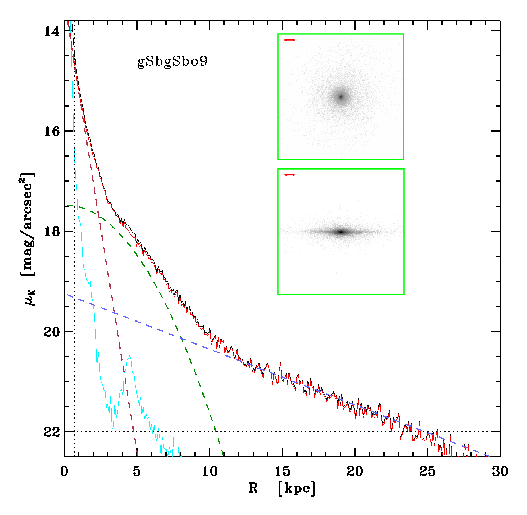
\includegraphics{Figures/aa24303-14-fig12.eps}
    \caption{Image of the light profile of a simulated S0 type galaxy. It shows how the intensity of light for the lenticular galaxy depends on the radius from the center. Querejeta et al 2015}
    \label{profile_fig}
\end{figure}
From observational evidence, one formation mechanism for S0 galaxies is ram-pressure stripping in galaxy clusters\citep{Querejeta_2015}. However, there are many S0 galaxies observed outside the confines of clusters, indicating that the ram-pressure stripping can't be the only formation mechanism and hence indicating mergers may be able to result in S0 galaxies.

%What question am I answering?
In this project, we intend to answer the question if a lenticular galaxy can be the result of a major merger between spiral galaxies. Currently, the full origin of Lenticular galaxies is not well known. From observations in galaxy surveys it is known S0-type galaxies are present inside and outside galaxy clusters. Thus their formation is not tied only to galaxy clsuters\citep{van_den_Bergh_2009} There may be more than one formation pathway to form S0 galaxies. Currently ,a number of research teams are studying the formation of S0-type galaxies using numerical simulations\citep{Querejeta_2015_2}. Simulations are about the only way this is possible because one needs to see the entire merger process.

%As of the present, the formation history of lenticular galaxies is still not well understood. Their rotation and dynamics and morphology are apparently intermediate of the spiral and elliptical galaxies. This hints at their origin as merger remnants. It may be possible that the Milky Way and Andromeda merger remnant could at least initially be a lenticular galaxy before evolving further into an elliptical galaxy. This type of evolution can be studied using dynamical simulations, namely n-body simulations. The details of the n-body simulations I will use are elaborated in the paper by van der Marel et. al \citep{van_der_Marel_2012_1,Sohn_2012}.

\section{This Project}
This research project intends to explore if the merger remnant of the Milky Way and Andromeda galaxies could be an S0-type galaxy. The origin of the S0 galaxies is interesting since they are an unusual type of galaxy. In connection to this question, I will also explore if the remnant of the merger is a slow or fast rotator. This could be a sign of an S0-type galaxy. If there is significant rotation in the merger remnant, it could be a sign that it is S0-type since an elliptical galaxy would not have significant net rotation.

A lead research question this study aims to address is if the S0-type galaxies could be the result of a major merger outside an environment of a galaxy cluster. One hypothesis for the lenticular galaxy formation is that they could be spirals whose gas was ram-pressure striped as they passed through a cluster. However lenticular galaxies are also observed far from clusters as well. Using the merger of the Milky Way and Andromeda galaxies as an example of a major merger between spiral galaxies, the remnant will be probed to determine if it is of type S0.

This study addresses the open question of lenticular galaxy formation outside galaxy cluster environments. Since the final product of a major merger is expected to be an elliptical galaxy, this study may show that a lenticular is merely an intermediate stage in the merger process as the merger remnant evolves into a true elliptical galaxy. However, the possibility of a lenticular galaxy evolving into an elliptical will not be answered since this would rely on a study of how the gas in the disk is heated up and/or dissipates. 

%In order to identify if the merger remnant is a lenticular galaxy (S0) it will be necessary to fit the light profile. I will attempt to do this by assuming an average luminosity value for the stellar particles in the simulation and integrating the light within a given radius. This will result in a graph like that in the introduction\ref{profile_fig}\cite{Querejeta_2015}. I will want to search for a new population of the bulge and disk stars if this remnant is an S0 type. This is illustrated in \ref{fig_2}. The red bulge area should have different dynamics than the disk that is enclosed in the green circle. I will try to explore this also by trying to plot the rotation speed of both components. I will try to search for a large slow rotating bulge and a faster-rotating disk. A change in the velocity dispersion between the bulge and disk will also indicate the S0 type.

%There is some evidence that the mergers of similar mass large galaxies can produce lenticular galaxies \citep{Querejeta_2015}. However, this seems to be a rather tentative result so I don't expect a perfect S0 identification. I will hope for some sign that the tidal tales can orbit to become a disk and hence form an S0 galaxy. I personally expect that S0 galaxies are a short-lived phase for a galaxy. It may happen that the merger remnant may initially resemble an S0 type but the disk could disperse and result in a more classical elliptical galaxy at later times in the simulation.

\section{Methodology}
%N-body simulations
In this project, the merger between the Milky Way and the Andromeda Galaxy is explored using N-body simulations. The N-body simulations used were created by van der Marel et. al. \cite{van_der_Marel_2012_1,van_der_Marel_2012_2} Of the Local Group galaxies in only the Milky Way, M31 and M33 are present in the simulation. Each galaxy is divided into three components, disk stars, bulge stars, and dark matter. The gravitational forces between each particle of mass are calculated according to Newton's theory of gravity. Then, due to the acceleration of gravity, the positions and velocities of each particle are updated.  In the simulation, this process is run for 800 Myrs of simulation time.

%Overview of Approach
The goal of this project is to determine if the merger remnant of the Milky Way and Andromeda is a lenticular galaxy. In order to do this Sersic profiles will be fit to merger remnant. For the sake of simplicity, the mass-to-light ratio will be taken as one. Then a combination of Sersic profiles of different indices will be fit to the remnant. From this fitted profile it will be examined to see if there is a distinct contribution from a disk and bulge. As a sanity check the rotational velocity as a function of the radius will be plotted. If appreciable rotation is observed then this indicates that there may be a rotating disk. 

 \begin{figure}
     \centering
     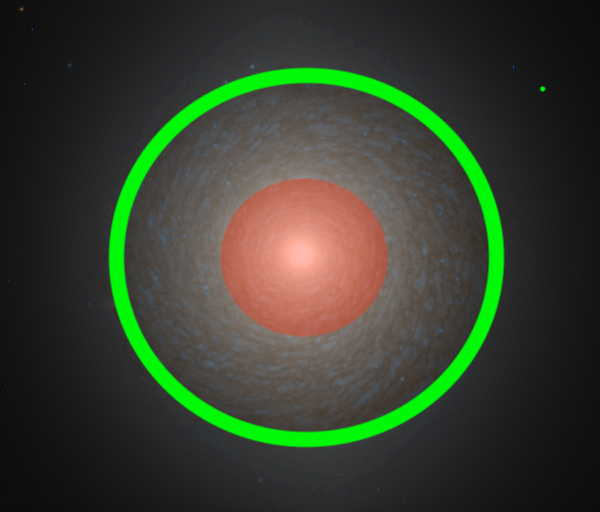
\includegraphics[scale=0.35]{Figures/NGC1387_-_hst_10217R850GB475.png}
     \caption{This is an image of an S0 galaxy with color overlays indicating the bulge and disk components. A Sersic profile will be fitted to both components to determine if it is a lenticular galaxy.}
     \label{fig_2}
 \end{figure}

 The main task of the code that is being written is to fit Sersic profiles to the merger remnant of the Milky Way and Andromeda. I will take the mass to light ratio to be unity to simplify the project. The method used to fit the profiles relies on the fact that disks and elliptical bulges have different profile functions. The sum of a disk and bulge profile will be fit and if the contribution from the disk is negligable than the remnant is likely elliptical and not lenticular. The equation for a Sersic profile is:
 \begin{equation}
     I(r) = I_0e^{-(r/h)^{1/n}},
 \end{equation}
 where $I$ is the intensity, $I_0$ is the central brightness, $r$ is the radius, $h$ is the scale length, and $n$ is the index. For an elliptical galaxy the index is $4$ and for a spiral disk the index is $1$. A sum of these profiles will be fit to see if the galaxy has both a bulge and disk.

 The first plot made by this project will be a graph of intensity vs radius. This graph will show the intensity vs radius for the galaxy from the data and the fitted Sersic profiles. Since a numpy fitting function will be used, the profile should match the data very closely. The second plot will be of circular speed as a function of radius. This will be a sanity check to see if there is appreciable rotation in the merger remnant.

 Since a lenticular galaxy is a fairly rare type of galaxy I would be surprised if the remnant is actually a lenticular galaxy. I suspect that remnant will be best described by a single Sersic profile of index of about four. This would mean that the remnant is an elliptical galaxy. However if the result is of type S0 there will be a contribution to the light profile from a Sersic profile of index 1. 

% \subsection{Figures and tables}

% Figures and tables should be placed at logical positions in the text. Don't
% worry about the exact layout, which will be handled by the publishers.

% Figures are referred to as e.g. Fig.~\ref{fig:example_figure}, and tables as
% e.g. Table~\ref{tab:example_table}.

% % Example figure
% \begin{figure}
% 	% To include a figure from a file named example.*
% 	% Allowable file formats are eps or ps if compiling using latex
% 	% or pdf, png, jpg if compiling using pdflatex
% 	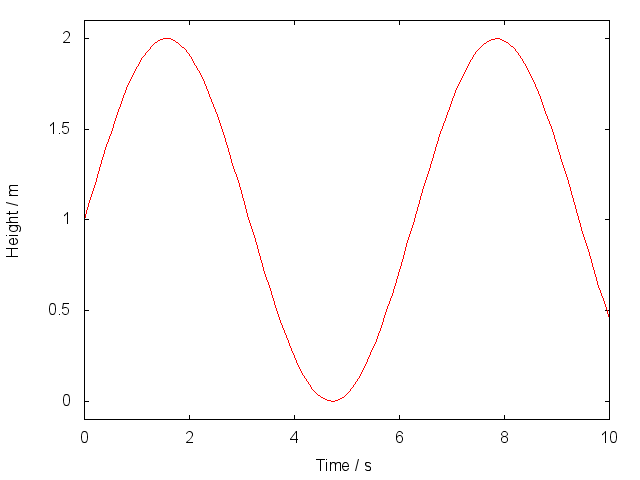
\includegraphics[width=\columnwidth]{example}
%     \caption{This is an example figure. Captions appear below each figure.
% 	Give enough detail for the reader to understand what they're looking at,
% 	but leave detailed discussion to the main body of the text.}
%     \label{fig:example_figure}
% \end{figure}

% % Example table
% \begin{table}
% 	\centering
% 	\caption{This is an example table. Captions appear above each table.
% 	Remember to define the quantities, symbols and units used.}
% 	\label{tab:example_table}
% 	\begin{tabular}{lccr} % four columns, alignment for each
% 		\hline
% 		A & B & C & D\\
% 		\hline
% 		1 & 2 & 3 & 4\\
% 		2 & 4 & 6 & 8\\
% 		3 & 5 & 7 & 9\\
% 		\hline
% 	\end{tabular}
% \end{table}


% \section{Conclusions}

% The last numbered section should briefly summarise what has been done, and describe
% the final conclusions which the authors draw from their work.

% \section*{Acknowledgements}

% The Acknowledgements section is not numbered. Here you can thank helpful
% colleagues, acknowledge funding agencies, telescopes and facilities used etc.
% Try to keep it short.

% %%%%%%%%%%%%%%%%%%%%%%%%%%%%%%%%%%%%%%%%%%%%%%%%%%
% \section*{Data Availability}

 
% The inclusion of a Data Availability Statement is a requirement for articles published in MNRAS. Data Availability Statements provide a standardised format for readers to understand the availability of data underlying the research results described in the article. The statement may refer to original data generated in the course of the study or to third-party data analysed in the article. The statement should describe and provide means of access, where possible, by linking to the data or providing the required accession numbers for the relevant databases or DOIs.




%%%%%%%%%%%%%%%%%%%% REFERENCES %%%%%%%%%%%%%%%%%%

% The best way to enter references is to use BibTeX:

\bibliographystyle{mnras}
\bibliography{example} % if your bibtex file is called example.bib


% Alternatively you could enter them by hand, like this:
% This method is tedious and prone to error if you have lots of references
%\begin{thebibliography}{99}
%\bibitem[\protect\citeauthoryear{Author}{2012}]{Author2012}
%Author A.~N., 2013, Journal of Improbable Astronomy, 1, 1
%\bibitem[\protect\citeauthoryear{Others}{2013}]{Others2013}
%Others S., 2012, Journal of Interesting Stuff, 17, 198
%\end{thebibliography}

%%%%%%%%%%%%%%%%%%%%%%%%%%%%%%%%%%%%%%%%%%%%%%%%%%

%%%%%%%%%%%%%%%%% APPENDICES %%%%%%%%%%%%%%%%%%%%%

\appendix

\section{Some extra material}

If you want to present additional material which would interrupt the flow of the main paper,
it can be placed in an Appendix which appears after the list of references.

%%%%%%%%%%%%%%%%%%%%%%%%%%%%%%%%%%%%%%%%%%%%%%%%%%


% Don't change these lines
\bsp	% typesetting comment
\label{lastpage}
\end{document}

% End of mnras_template.tex
